\documentclass[class=report, crop=false, 12pt,a4paper]{standalone}
\usepackage{enumitem}
\usepackage{multicol}
\usepackage{etoolbox}
\AtBeginEnvironment{quote}{\singlespacing\small}
\usepackage{setspace}
\onehalfspacing
\usepackage{graphicx}
\usepackage{float}
\usepackage{amsmath}
\usepackage{amssymb}
\usepackage{siunitx}
\sisetup{detect-all}
\begin{document}
\section{Gas power cycles}
\subsection{Thermodynamic cycles}
Two important areas of application of thermodynamics are power generation and refrigeration. Both are accomplished by systems that operate on a thermodynamic cycle.
\begin{itemize}[noitemsep]
  \item Power cycles: operated as engines.
  \item Refrigeration cycles: operated as refrigerators, air conditioners, heat pumps, etc.
  \item Gas cycles: the working fluid remains in the gaseous phase throughout the entire cycle.
  \item Vapour cycles: the working fluid exists in the vapour phase during part of the cycle and in the liquid phase during another part. 
  \item Closed cycles: the working fluid is returned to the initial state at the end of the cycle and is recirculated.
  \item Open cycles: the working fluid is renewed at the end of the cycled instead of being recirculated.
\end{itemize}
\subsection{Heat engines}
In automobile engines, the combustion gases are exhausted and replaced by the fresh air-fuel mixture at the end of each cycle. The engine operates on a mechanical cycle but the working fluid does not go through a complete thermodynamic cycle. 
\begin{itemize}[noitemsep]
  \item Internal combustion engine: heat is supplied by burning the fuel within the system boundaries e.g. automobile engines.
  \item External combustion engine: heat is supplied to the working fluid from an external source such as a furnace e.g. steam power plants.
\end{itemize}
\subsection{Basic considerations in the analysis of power cycles}
The cycles encountered in actual devices are difficult to analyse because of the presence of complicating effects such as friction and the absence of sufficient time for establishment of the equilibrium conditions during the cycle. Thus, we utilise some idealisations. An ideal cycle is an actual cycle stripped of all its internal irreversibilities, producing a graph made up totally of internally reversible processes. The ideal cycle can be used to show the general characteristics. Recall,
\begin{align}
  \eta_{th} &= \frac{W_{net}}{Q_{in}} \textrm{ or}\\
  \eta_{th} &- \frac{w_{net}}{q_{in}} 
\end{align}
\begin{figure}[h]
  \centering
  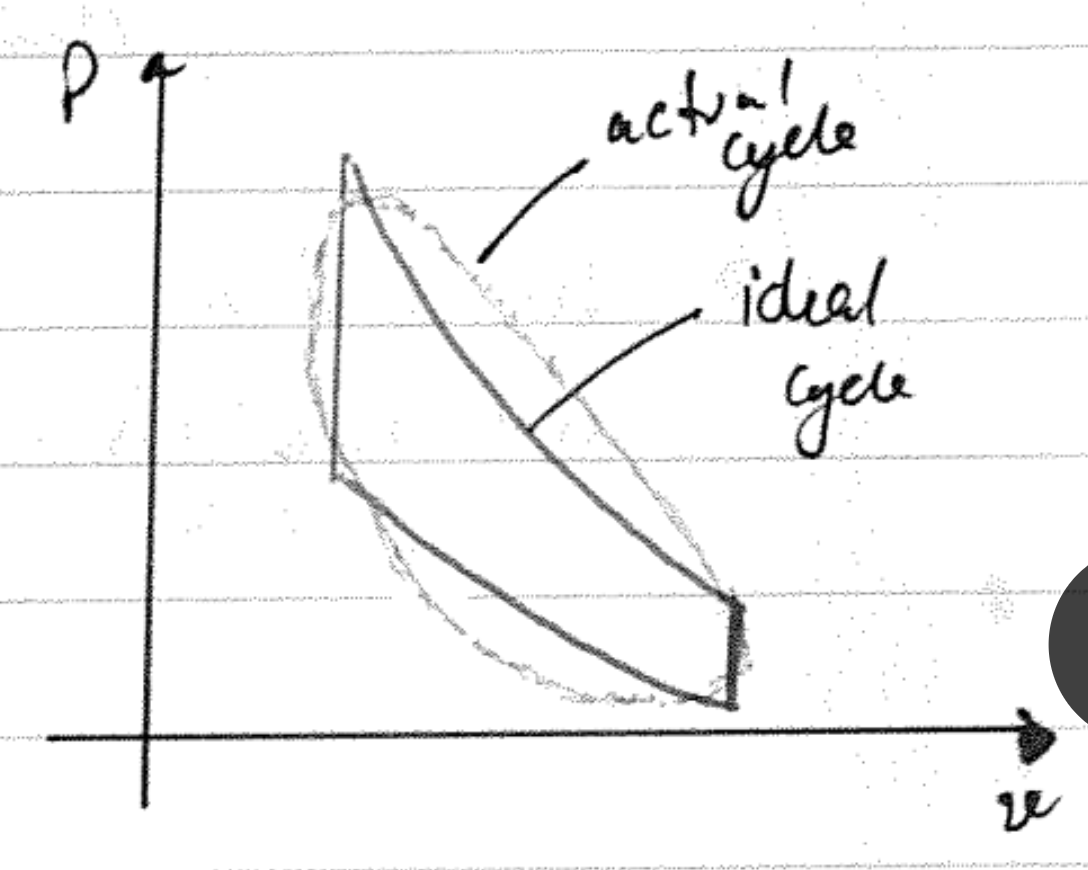
\includegraphics[width = 0.5\textwidth]{../img/actualvsidealcycle}
  \caption{How an ideal cycle compares to the actual cycle.}
  \label{fig:actualvsidealcycle}
\end{figure}
Also, heat engines on a totally reversible cycle (such as the Carnot cycle) have the highest thermal efficiency of all heat engines operating between the same temperature levels. The question arises: why do we not use the Carnot cycle? This is due to hardware. It is difficult to implement it. Thus, other ideal cycles are used.
\begin{equation}
  \eta_{th, \textrm{ totally reversible}} > \eta_{th, \textrm{ internally reversible}} = \eta_{th, \textrm{ ideal gas}}
\end{equation}
This applies between the same temperature limits. We also have:
\begin{equation}
  \eta_{th, \textrm{ ideal cycle}} > \eta_{th, \textrm{ actual cycle}}
\end{equation}
The idealisations and simplifications commonly employed in the analysis of power cycles can be summarised as follows:
\begin{enumerate}[noitemsep]
  \item The cycle does not involve any friction. Thus, the working fluid does not experience any pressure drop as it flows in pipes or devices such as heat exchangers.
  \item All expansion and compression processes take place in a quasi - equilibrium manner.
  \item The pipes connecting various components of a system are well insulated and heat transfer through them is negligible.
\end{enumerate}
Kinetic energy and potential energy are also generally neglected as their changes are negligible.
\begin{align}
  \textrm{KE and PE neglected for} & \begin{cases}
    \textrm{turbines}\\
    \textrm{compressors}\\
    \textrm{pumps}
  \end{cases}\\
  \textrm{KE neglected for} & \begin{cases}
    \textrm{condensers}\\
    \textrm{boilers}\\
    \textrm{mixing chambers}
  \end{cases}\\
  \textrm{KE not neglected for} & \begin{cases}
    \textrm{nozzles}\\
    \textrm{diffusers}
  \end{cases}
\end{align}
Also, note that for P-V and T-S diagrams, the area enclosed, for both, is the net work produced during a cycle.
\subsection{T-S diagram tips and tricks}
\begin{itemize}[noitemsep]
  \item A heat - addition process proceeds in the direction of increasing entropy. 
  \item A heat - rejection process proceeds in the direction of decreasing entropy. 
  \item An isentropic (internally reversible, adiabatic) process proceeds at constant entropy. 
  \item The area under the process curve on a T-S diagram represents the heat transfer for that process.
\end{itemize}
\subsection{The Carnot cycle and its value in engineering}
\begin{equation}
  \eta_{th, \textrm{ Carnot}} = 1 - \frac{Q_L}{Q_H} = 1 - \frac{T_L}{T_H}
  \label{carnotefficiency}
\end{equation}
Thermal efficiency increases with an increase in the average temperature at which heat is supplied to the system, or with a decrease in the average temperature at which heat is rejected from the system. The highest temperature in the cycle is limited by the maximum temperature that the components of the heat engine, such as the piston or the turbine blades, can withstand. The lowest temperature is limited by the temperature of the cooling medium utilised in the cycle such as a lake, a river or the atmospheric air.
\subsubsection{Proof question}
Show that the thermal efficiency of a Carnot cycle operating between the temperature limits $T_H$ and $T_L$ is solely a function of these two temperature and is given by equation \ref{carnotefficiency}.

Carnot cycle is:
\begin{enumerate}[noitemsep]
  \item Isothermal heat addition.
  \item Isentropic expansion.
  \item Isothermal heat rejection.
  \item Isentropic compression.
\end{enumerate}
\begin{figure}
  \centering
  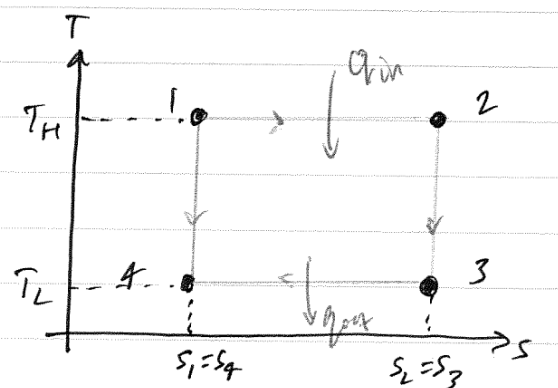
\includegraphics[width = 0.5\textwidth]{../img/carnotq}
  \caption{T-S diagram for Carnot cycle}
\end{figure}
\begin{align}
  q_{in} &= \textrm{Area under graph as processes are totally reversible}\\
  &= T_H(S_2 - S_1) = T_H(S_3 - S_4)\\
  q_{out} &= \textrm{Area under process 3-4}\\
  &= T_L(S_3 - S_4) = T_L(S_2 - S_1)\\
  \eta_{th} &= 1 - \frac{q_{out}}{q_{in}} = 1 - \frac{T_L(S_2 - S_1)}{T_H(S_2 - S_1)}\\
  \eta_{th, \textrm{ const}} &= 1 - \frac{T_L}{T_H}
\end{align}
\subsection{Air-standard assumptions}
\end{document}